%%
%% Author: Alexander Telich
%% 2/14/18
%%

% Preamble
\documentclass[11pt]{article}
\usepackage[utf8]{inputenc}
\usepackage{amsmath}

% Packages
\usepackage{a4wide}
\usepackage{listings}
\usepackage{indentfirst}
\usepackage{graphicx}

\lstdefinestyle{mystyle}{
basicstyle=\footnotesize,
breakatwhitespace=false,
breaklines=true,
captionpos=b,
keepspaces=true,
numbers=left,
numbersep=5pt,
showspaces=false,
showstringspaces=false,
showtabs=false,
tabsize=2
}

\lstset{style=mystyle}

\author{Alexander Telich}
\title{EECS 531 A1 Exercise 2}
\date{February 14, 2018}
\graphicspath{C:/Users/ateli/Documents/School/Spring 2018/EECS 531/Assignments/531_A1/A1/Exercise2}

% Document
\begin{document}
    \maketitle
    \section{Canny Edge Detection}\label{sec:exercise1}
    \subsection{Noise Reduction}\label{subsec:1.NoiseReduction}
    \setlength\parindent{24pt}
    The first step in the Canny Edge Detection Algorithm is to remove the noise in the image
    with a 5x5 Gaussian filter.
    This was the same technique used in Exercise 1 to create the blurring filter.
    \subsection{Intensity Gradient of the Image}\label{subsec:2.IntensityGradientOfTheImage}
    \setlength\parindent{24pt}
    After the noise was reduced from the image, it was filtered with a Sobel kernel in
    the vertical and horizontal direction.
    The Sobel kernel is convolved with the source image in the horizontal and vertical
    directions by equations (1) and (2).
    \begin{equation}
        G_x=\left[\begin{matrix}+1&0&-1\\+2&0&-2\\+1&0&-1\\\end{matrix}\right]\ast\ Source\ Image
    \end{equation}
    \newline
    \begin{equation}
        G_y=\left[\begin{matrix}+1&+2&+1\\0&0&-2\\+1&-2&-1\\\end{matrix}\right]\ast\ Source\ Image
    \end{equation}
    \newline
    Then, the edge gradient was found by using the horizontal and vertical edge gradients,
    found in equations (1) and (2), in the following equation (3).
    \begin{equation}
        G=\sqrt{G_x^2+G_y^2}
    \end{equation}
    {\small \begin{center}
          where $G$ is the edge gradient\\
    \end{center}}
    \begin{equation}
        \theta=\tan^{-1}{\left(\frac{G_y}{G_x}\right)}
    \end{equation}
    {\small \begin{center}
                where $\theta$ is the gradient direction angle\\
    \end{center} }
    \newline
    Finally, because the gradient direction was measured on the horizontal and vertical axises
    of the image, the gradient direction was always perpendicular to the edges of the image.
    Therefore, it was rounded to one of four angles representing the 4 cardinal directions.
    \subsection{Non-maximum Suppression}\label{subsec:non-maximumSuppression}
    Once the gradient's magnitude and direction were calculated, the image was scanned to
    remove unwanted pixels that did not constitute the edge.
    At each pixel, the pixel was checked if it was a local maximum within the patch size
    in the direction of the gradient vector.
    \subsection{Hysteresis Thresholding}\label{subsec:hysteresisThresholding}
    In this stage, minimum and maximum values were decided to create a threshold.
    This threshold classified any edge with an intensity gradient greater than maxVal as edges.
    Any intensity gradient that fell below minVal were not classified as edges.
    An intensity gradient that was between the minVal and maxVal of the threshold were decided
    to be edges if they were connected to pixels that were above the maxVal.

    \section{Code}\label{sec:codeExplanation}
    \lstinputlisting[language=Python]{Exercise2.py}

    \begin{figure}[h]
    \caption{Original Image}
    \centering
    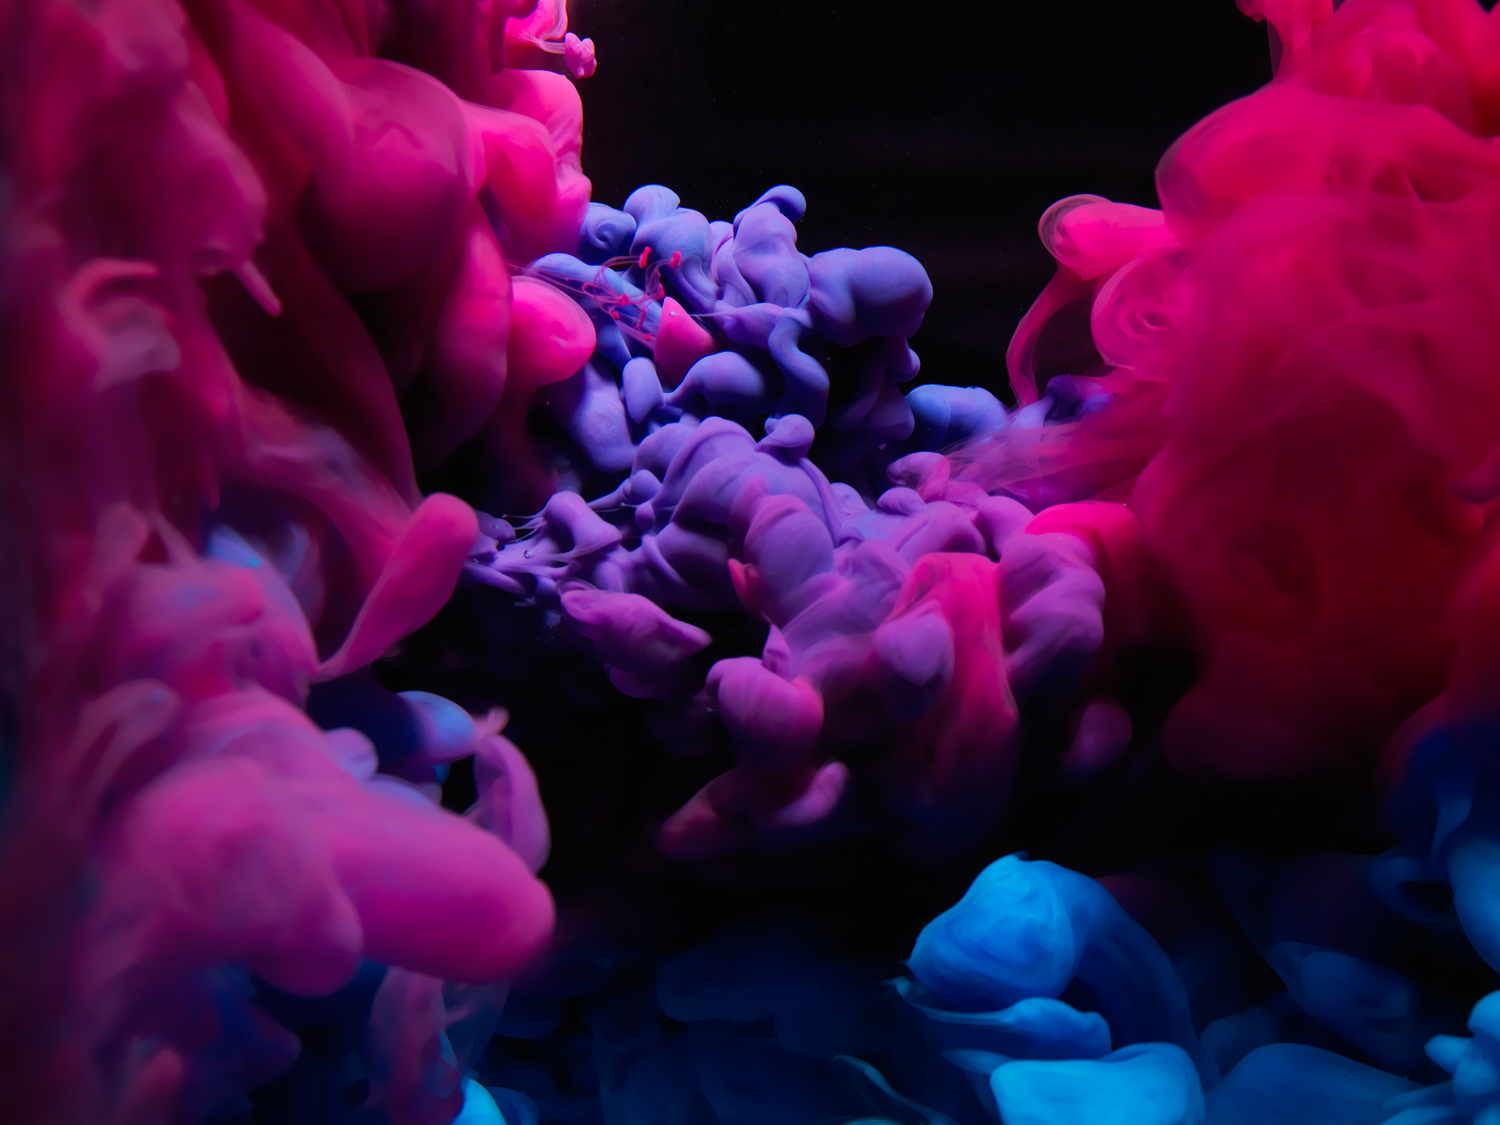
\includegraphics[scale=0.22]{Exercise2_Image.jpg}
    \end{figure}

    \begin{figure}[h]
    \caption{Image After Edge Processing}
    \centering
    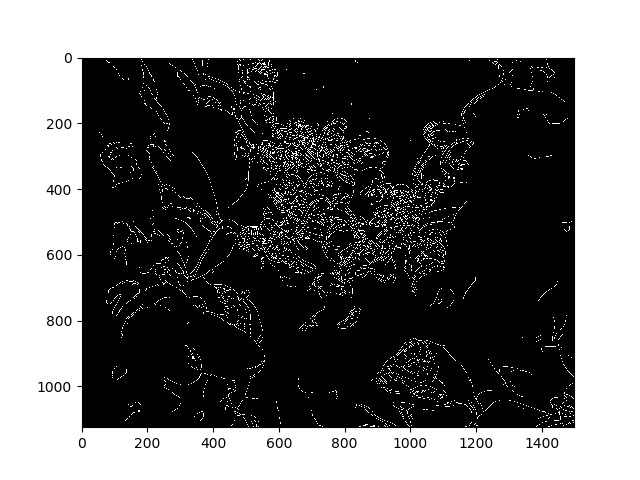
\includegraphics[scale=0.63]{myplot.png}
    \end{figure}

\end{document}
\begin{document}



\end{document}
\begin{document}



\end{document}